\chapter{基于多尺度网络结构的故障诊断模型研究}
\label{cha:chapter4}

\section{引言}

在第~\ref{cha:chapter3}章中,我们设计了一个结构与VGG类似的卷积神经网络模型来完成故障
模式的学习和预测。从该模型的结构示意图~\ref{fig:cnn_classifier}以及各层特征图的数据维
度变化图~\ref{fig:cnn_data}可以看出,在网络中的特征提取阶段,由于下采样层的存在,网络
每经过一个图~\ref{fig:cnn_classifier}中虚线框表示的基本单元,特征图在空间的尺寸就会减
半。我们知道,下采样层的作用是从输入数据中筛选出显著特征,因此经过多个下采样层之后,
输入数据的整体特征被提取出来,而局部特征被丢弃。这一点从~\ref{subsection:cascade_result}
节给出的实验结果也可以得到印证。在~\ref{subsection:cascade_result}中我们比较了不同核
宽度的平均值下采样提取的特征向量,这里我们将核宽度$F$分别等于2、4、8、16、32时,使用单
层平均值下采样提取的特征向量绘制成图~\ref{fig:features_scales}。可以看出,下采样程度
越大,提取的特征中保留的原始信号频谱序列的细节信息就越少。
\begin{figure}[ht]
  \centering
  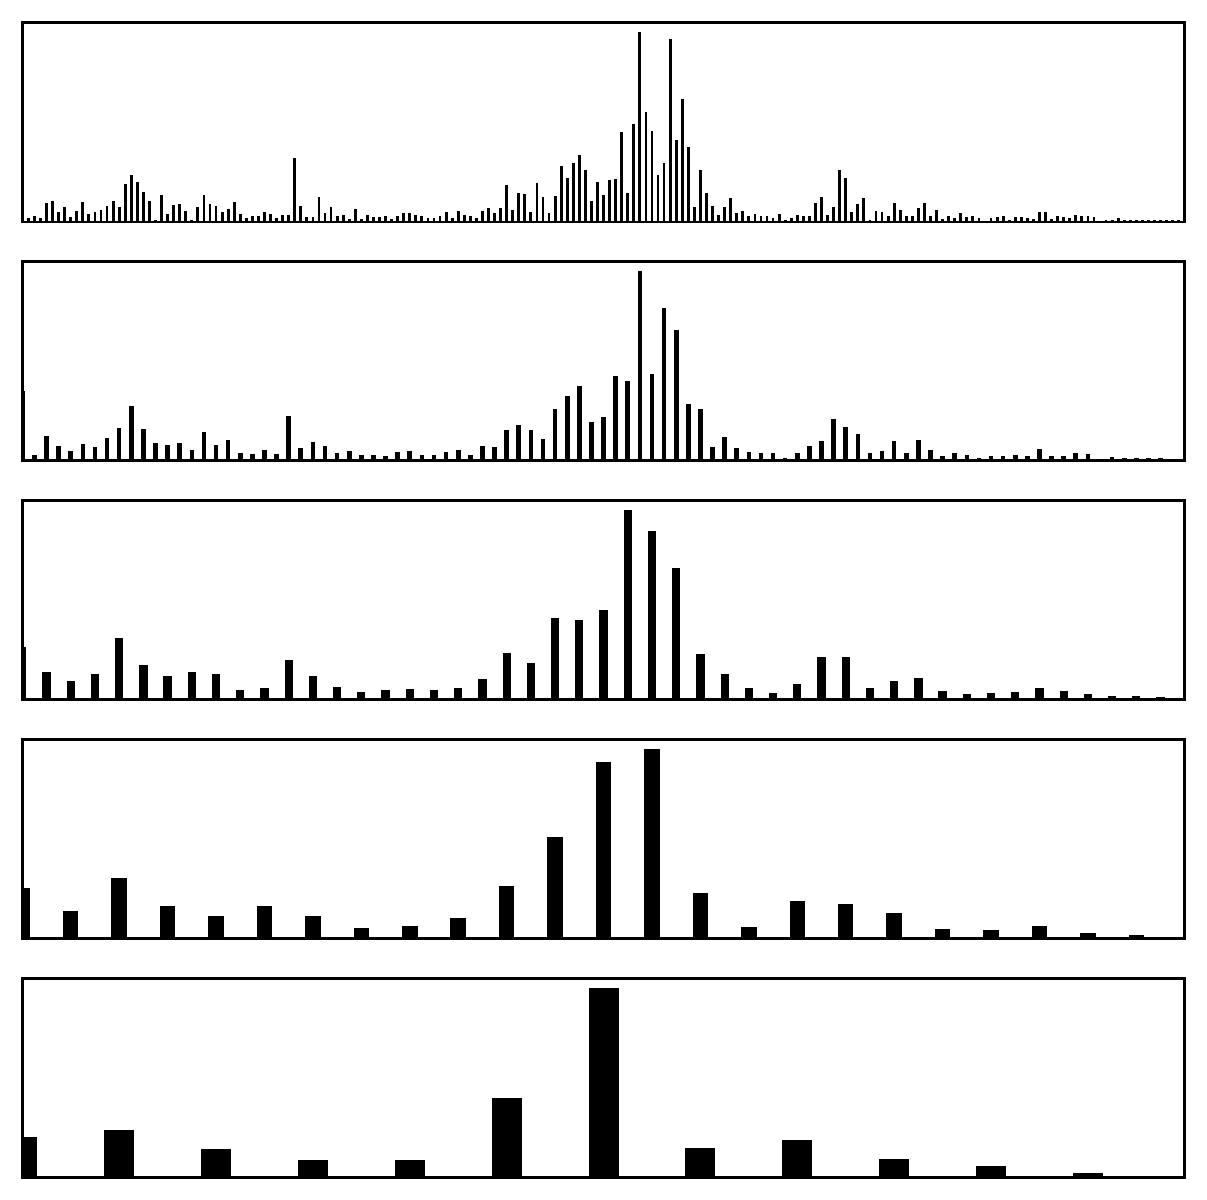
\includegraphics[height=10cm]{features_scales}
  \caption{不同采样程度下提取的特征向量}
  \label{fig:features_scales}
\end{figure}

总体上讲,这样的特征提取过程有助于分析输入数据和输出标签之间的联系,但是如果这些局部
特征在特征提取的过程中能够在一定程度上得到保留,或者是跟下采样得到的整体特征加以融合,
那么一定能够提升模型对输入数据的理解程度,从而提升模型最终的预测精度。

本章首先介绍了一个新的网络层——上采样(Upsampling)层。然后设计了一个递归的网络结构,
使得模型在特征提取阶段能够将经过下采样之后的整体特征和下采样前的局部特征进行融合,从
而使得模型最终提取的特征向量中也包含输入数据的细节信息。最后使用该模型在CWRU数据集上
进行实验验证,得到了比第~\ref{cha:chapter2}章和第~\ref{cha:chapter3}章都要更好的预测
精度。此外,本章还将实验中获得的结果与其他论文在该数据集上获得的效果进行了对比。

\section{上采样}

在~\ref{subsection:cnn}节中,我们介绍了卷积神经网络中经常使用的下采样层,输入数据在
经过下采样层之后空间的尺寸会减小。例如图片经过下采样之后图片的宽度和高度会减小,得到
分辨率更低的缩略图。我们也可以通过上采样操作向图片中添加像素,从而增大图片的尺寸。

上采样的过程实际上是通过插值算法来完成的,下面我们对使用最近邻插值算法进行上采样的
过程做简单介绍。例如我们要将原始图像放大3倍,那么图像中原本的像素位置随着图像尺寸的
变大而向外扩张,因此各行(列)像素间将会产生空隙,根据最近邻插值算法,我们可以使用离
得最近的像素值来填补这些空隙。也就是将原始图像中的每个像素值沿宽度和高度方向均重复3
次,变成$3\times 3$个像素。如图~\ref{fig:nn_upsampling}所示。
\begin{figure}[ht]
  \centering
  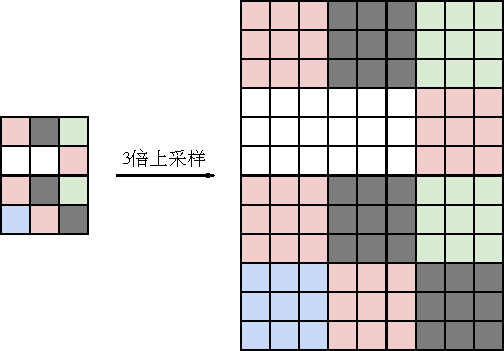
\includegraphics{nn_upsampling}
  \caption{最近邻插值算法示意图}
  \label{fig:nn_upsampling}
\end{figure}

除最近邻插值算法外,常见的还有双线性插值算法、双三次插值算法等。还有一些针对特定放大
比例的算法,例如在放大2倍、3倍或4倍时分别对应的hq2x、hq3x和hq4x算法等。图~\ref{fig:image_upsampling}
是不同插值算法在同一张图片上实现的上采样结果示例。
\begin{figure}[ht]
  \centering
  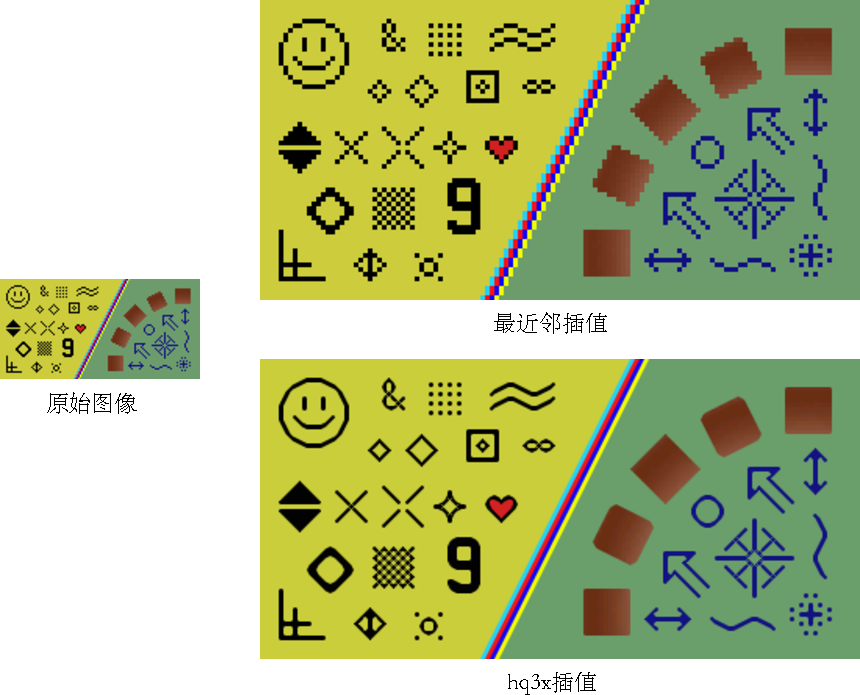
\includegraphics[width=12cm]{image_upsampling}
  \caption{两种插值算法在同一张图片上的上采样结果示例}
  \label{fig:image_upsampling}
\end{figure}

在卷积神经网络中,同下采样层一样,上采样层也是独立操作特征图深度方向上的每一个切片,
用指定的插值算法来对每个切片在空间上的尺寸进行放大。上采样层同样也不改变特征图的深度,
并且也不会向网络中引入参数。一般地,如果上采样层输入的特征图维度为
$W_1\times H_1\times D_1$,放大比例为$S$,输出的特征图维度为$W_2\times H_2\times D_2$,
那么有:
\begin{equation}
  \label{equ:chap4:upsampling_dim}
  \left\{\begin{aligned}
    & W_2 = W_1 \cdot S \\
    & H_2 = H_1 \cdot S \\
    & D_2 = D_1
  \end{aligned}\right.
\end{equation}

\section{基于多尺度网络结构的故障诊断模型}

第~\ref{cha:chapter3}章中使用连续的多个卷积层+ReLU层+下采样层顺序相连的网络模型
对输入信号频谱序列进行了特征提取和分类。本章在网络中加入了上采样层,并设计了一种
多尺度的网络结构,使得网络中下采样之后和下采样之前两种尺度的特征能够进行融合,从而
能够同时保留整体和局部特征,提升网络对输入数据的理解能力。网络的基本构成单元如图~\ref{fig:ms_unit}
所示。

\begin{figure}[ht]
  \centering
  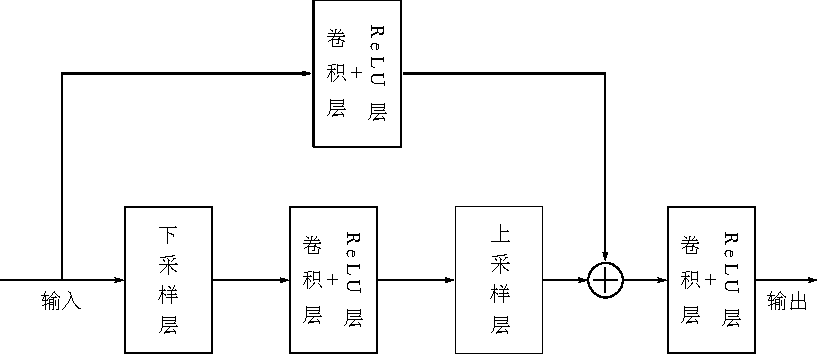
\includegraphics{ms_unit}
  \caption{多尺度网络结构的基本构成单元}
  \label{fig:ms_unit}
\end{figure}

从图中可以看出,输入数据在网络中被分为两个分支,一个为下采样之后低分辨率(空间尺寸
被压缩)的分支,另一个是下采样之前高分辨率(空间尺寸未被压缩)的分支。这两个分支各
自经过卷积层和ReLU层的处理,之后将低分辨率分支的结果进行上采样,并将上采样的结果与
高分辨率分支的结果相加。最后两个分支相加的结果在经过卷积层和ReLU层的处理之后作为网
络单元的输出。

图~\ref{fig:ms_unit}只是本章设计的多尺度网络基本连接方式的一个示意图,我们可以根据
问题的复杂程度对图~\ref{fig:ms_unit}进行一些适当的调整。例如我们可以在低分辨率分支
的上采样层和下采样层之间连接多个卷积层和ReLU层,同样也可以在高分辨率分支连接不止一
个卷积层和ReLU层。此外,由于两个分支在相加的时候必须保证各自分支上的数据维度一致,
因此最简单的方法就是让图~\ref{fig:ms_unit}中所有的卷积层的卷积核个数相同,这样在经
过每个卷积层之后都不会改变数据的维度。当然,我们也可以根据情况做一些调整。例如我们
可以在两个分支使用卷积核个数不同的卷积层,这时两个分支的数据在深度方向的维度将不再
一致,那么我们在对两个分支的数据进行相加操作之前,可以额外增加一个卷积层对分支的数
据维度进行适配。

从图~\ref{fig:ms_unit}中可以看出,由于下采样层和上采样层的存在,输入数据在空间上的
尺寸和输出数据在空间上的尺寸是保持一致的。

到目前为止,我们已经能够通过图~\ref{fig:ms_unit}所示的结构融合两种尺度下的特征,那
么如何利用多个这样的基本单元来构建一个网络,使得网络的输出能够融合多种尺度下的特征
呢?首先我们来说明图~\ref{fig:ms_seq_connected}所示的顺序连接方式是不可行的。
\begin{figure}[ht]
  \centering
  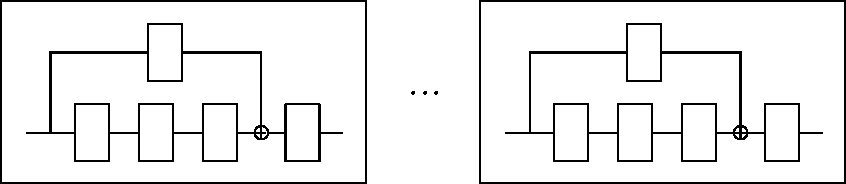
\includegraphics[width=12cm]{ms_seq_connected}
  \caption{多个基本单元顺序连接示意图}
  \label{fig:ms_seq_connected}
\end{figure}

从图~\ref{fig:ms_seq_connected}中可以看出,由于每个基本单元中均存在一个下采样层和
一个对应的上采样层,每个单元输入数据和输出数据在空间上的尺寸是相同的,因此多个这样
的单元顺序连接构建的网络中,从网络的输入到最后的输出之间,网络中流动的数据只有两种
尺度,达不到融合多尺度特征的目的。要想在网络中存在多种尺度的特征,必须在上采样
之前经过多次的下采样,也就是需要一个递归的连接方式来构造网络。如图~\ref{fig:cnn_ms}
所示。
\begin{figure}[ht]
  \centering
  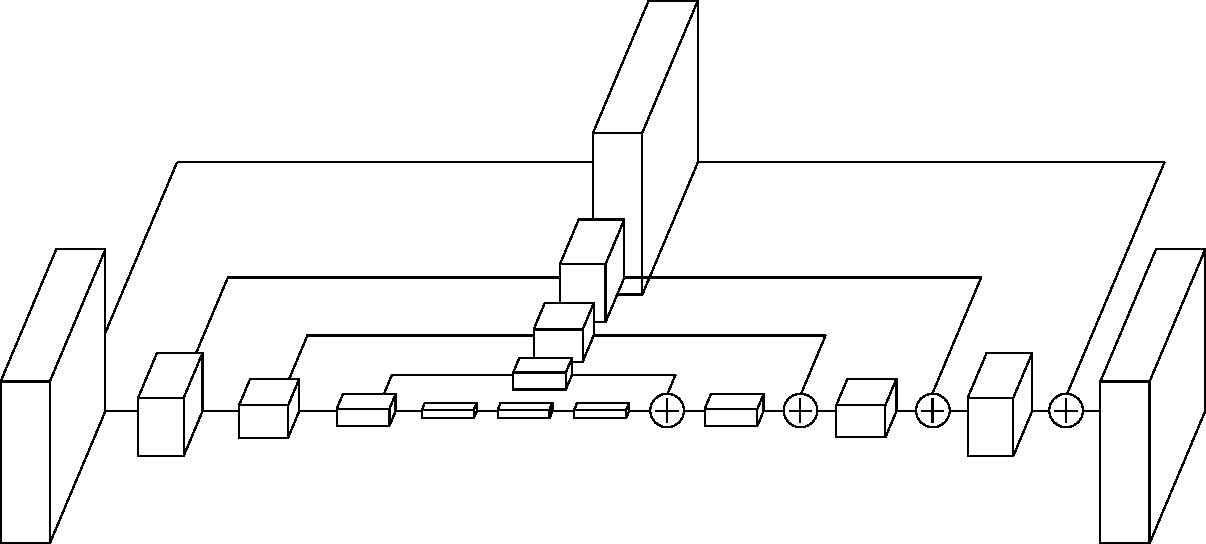
\includegraphics[width=13cm]{cnn_ms}
  \caption{多尺度网络结构的故障诊断模型}
  \label{fig:cnn_ms}
\end{figure}

图~\ref{fig:cnn_ms}中各个立方体块均表示特征图,可以看出这样的网络结构可以通过一个
多层递归过程来完成。在每一层递归中,对输入数据的处理都分为两个分支:下面的分支在
经过下采样层、卷积层、ReLU层之后,将结果作为下一层递归的输入,而下一层递归的输出
经过卷积层、ReLU层和上采样层之后与上面分支的结果相加,并将相加的结果作为输出返回
上一层递归。上面的分支处理过程比较简单,仅有卷积层和ReLU层构成。

下面用一段伪代码来描述图~\ref{fig:cnn_ms}所示的网络的构造过程。

\begin{algorithm}[ht]
    \caption{递归地构造多尺度网络}
    \begin{algorithmic}[1] %每行显示行号
        \Require $data$输入特征图,$n$递归次数
        \Ensure 输出特征图
        \Function {MultiScaleNet}{$data, n$}
						\State $up \gets \Call{Conv}{data}$
            \State $up \gets \Call{Relu}{up}$
            \State $low \gets \Call{MaxPooling}{data}$
            \State $low \gets \Call{Conv}{low}$
            \State $low \gets \Call{Relu}{low}$
            \If {$n > 1$}
                \State $low \gets \Call{MultiScaleNet}{low, n-1}$
						\Else
							\State $low \gets \Call{Conv}{low}$
							\State $low \gets \Call{Relu}{low}$
            \EndIf
						\State $low \gets \Call{Conv}{low}$
						\State $low \gets \Call{Relu}{low}$
						\State $low \gets \Call{Upsampling}{low}$
            \State \Return{$up + low$}
        \EndFunction
    \end{algorithmic}
\end{algorithm}

\section{实验验证}

\subsection{实验过程}

从图~\ref{fig:cnn_ms}中可以看出,虽然在多尺度网络内部存在着多种尺度的特征,但是网络
整体的输入和输出特征的空间维度是相等的。因此在实验中,我们并不是直接将信号频谱序
列输入到多尺度网络中,而是先经过一定数目的卷积层+ReLU层+下采样层的处理之后,再连接
一个多尺度网络,同样在多尺度网络之后也连接一定数目的卷积层+ReLU层+下采样层,最后使
用一个全连接层来对提取的特征进行分类。整个模型中各层节点数据的变化情况如图~\ref{fig:cnn_ms_data}
所示。
\begin{figure}[ht]
  \centering
  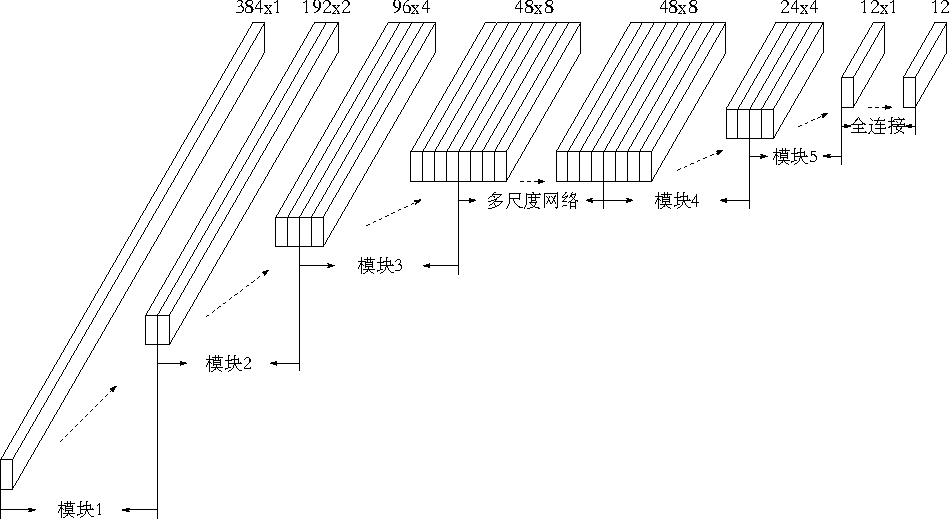
\includegraphics[width=13cm]{cnn_ms_data}
  \caption{基于多尺度网络的模型各层数据维度变化情况}
  \label{fig:cnn_ms_data}
\end{figure}

图~\ref{fig:cnn_ms_data}中模块1-5同样表示卷积层+ReLU层+下采样层的结构,各模块中卷
积层和下采样层的参数仍旧与表~\ref{tab:layer_parameters}中所列的参数一样。网络的输入
是信号片段的频谱序列$X$,维度为384。经过模块1、模块2和模块3之后,网络中的特征图维度
变为$48\times 8$;然后将这$48\times 8$的特征图输入到多尺度网络模块中进行处理,由于多
尺度网络模块并不改变特征的维度,因此输出的特征图维度仍为$48\times 8$;此后我们通过模
块4和模块5对特征的个数进行一定程度的压缩,最后通过一个全连接层进行故障分类。

\subsection{实验结果及分析}

仍然使用表~\ref{tab:class_desc}中所列的12类数据对本章提出的基于CNN的多尺度故障诊断
方法进行训练和测试,表~\ref{tab:chap4:classification_report}给出了模型在测试集上各
类的精确率、召回率、F1-Score等评价指标。
\begin{table}[htb]
  \centering
  \begin{minipage}[t]{0.8\linewidth}
  \caption{基于多尺度网络的故障诊断模型在测试集上的混淆矩阵}
  \label{tab:chap4:classification_report}
    \begin{tabularx}{\linewidth}{XXXXX}
      \toprule[1.5pt]
        故障类型    & 精确率 & 召回率 & F1-Score \\
      \midrule[1pt]
        正常        & 1.0000 & 1.0000 & 1.0000 \\
        钢球, 0.007 & 0.9915 & 0.9901 & 0.9908 \\
        钢球, 0.014 & 0.9949 & 0.9949 & 0.9949 \\
        钢球, 0.021 & 0.9936 & 0.9949 & 0.9943 \\
        钢球, 0.028 & 1.0000 & 1.0000 & 1.0000 \\
        内圈, 0.007 & 1.0000 & 1.0000 & 1.0000 \\
        内圈, 0.014 & 1.0000 & 1.0000 & 1.0000 \\
        内圈, 0.021 & 1.0000 & 1.0000 & 1.0000 \\
        内圈, 0.028 & 1.0000 & 1.0000 & 1.0000 \\
        外圈, 0.007 & 1.0000 & 1.0000 & 1.0000 \\
        外圈, 0.014 & 1.0000 & 1.0000 & 1.0000 \\
        外圈, 0.021 & 1.0000 & 1.0000 & 1.0000 \\
      \midrule[1pt]
        平均(总计)& 0.9985 & 0.9985 & 0.9985 \\
      \bottomrule[1.5pt]
    \end{tabularx}
  \end{minipage}
\end{table}

从表~\ref{tab:chap4:classification_report}可以看出,本章提出的基于CNN的多尺度故障
诊断方法在CWRU数据集上对轴承的12种故障状态的识别率可以达到99.85\%,分别比第~\ref{cha:chapter2}
章和第~\ref{cha:chapter3}章获得的识别率提升了8.85\%和2.49\%。此外,对于第~\ref{cha:chapter2}
章中预测效果比较差的三类故障样本,钢球部位0.007英寸、0.014英寸以及0.021英寸,本章
的模型在测试集上的F1-Score分别为99.08\%、99.49\%和99.43\%,分别比第~\ref{cha:chapter2}
章中对应的值提升了34.52\%、31.36\%和45.20\%,比第~\ref{cha:chapter3}章中对应的值提
升了16.83\%、6.28\%和13.07\%。除这三种故障样本之外,在其他类型的样本F1-Score都达到
了100.00\%。

为了与其他常见的多尺度的故障诊断方法进行比较,本文以表~\ref{tab:class_desc}所列
的12类数据为输入,经过RDFT变换的预处理之后,分别使用多尺度熵(MSE)、多尺度模糊
熵(MFE)、复合多尺度模糊熵(CMFE)、使用多尺度形态梯度分析(MMA)进行特征提取,
并在此基础上训练Softmax分类器,最后将各种方法在测试集上的平均精确率、平均召回率
和平均F1-Score列在表~\ref{tab:chap4:comparison}中,其中本章提出的基于CNN的多尺度
故障诊断方法简记为MS-CNN。
\begin{table}[htb]
  \centering
  \begin{minipage}[t]{0.8\linewidth}
  \caption{不同多尺度方法诊断效果比较}
  \label{tab:chap4:comparison}
    \begin{tabularx}{\linewidth}{XXXX}
      \toprule[1.5pt]
        方法名称 & 精确率 & 召回率 & F1-Score \\
      \midrule[1pt]
        MSE      & 0.9421 & 0.9169 & 0.9021 \\
        MFE      & 0.9457 & 0.9315 & 0.9282 \\
        CMFE     & 0.9494 & 0.9378 & 0.9395 \\
        MMA      & 0.9259 & 0.8994 & 0.8837 \\
        MS-CNN*  & 0.9985 & 0.9985 & 0.9985 \\
      \bottomrule[1.5pt]
    \end{tabularx}
  \end{minipage}
\end{table}

从表~\ref{tab:chap4:comparison}中可以看出,与其他一些多尺度的故障诊断方法相比,本章
提出的基于CNN的多尺度故障诊断方法在故障诊断精度上有比较大的优势。将图~\ref{fig:series}
中展示的$12\times 3$个信号频谱序列输入到训练好的网络中,得到本章的故障诊断方法提取的
融合了多种尺度下特征的向量,如图~\ref{fig:ms_cnn_features}所示。
\begin{figure}[ht]
  \centering
  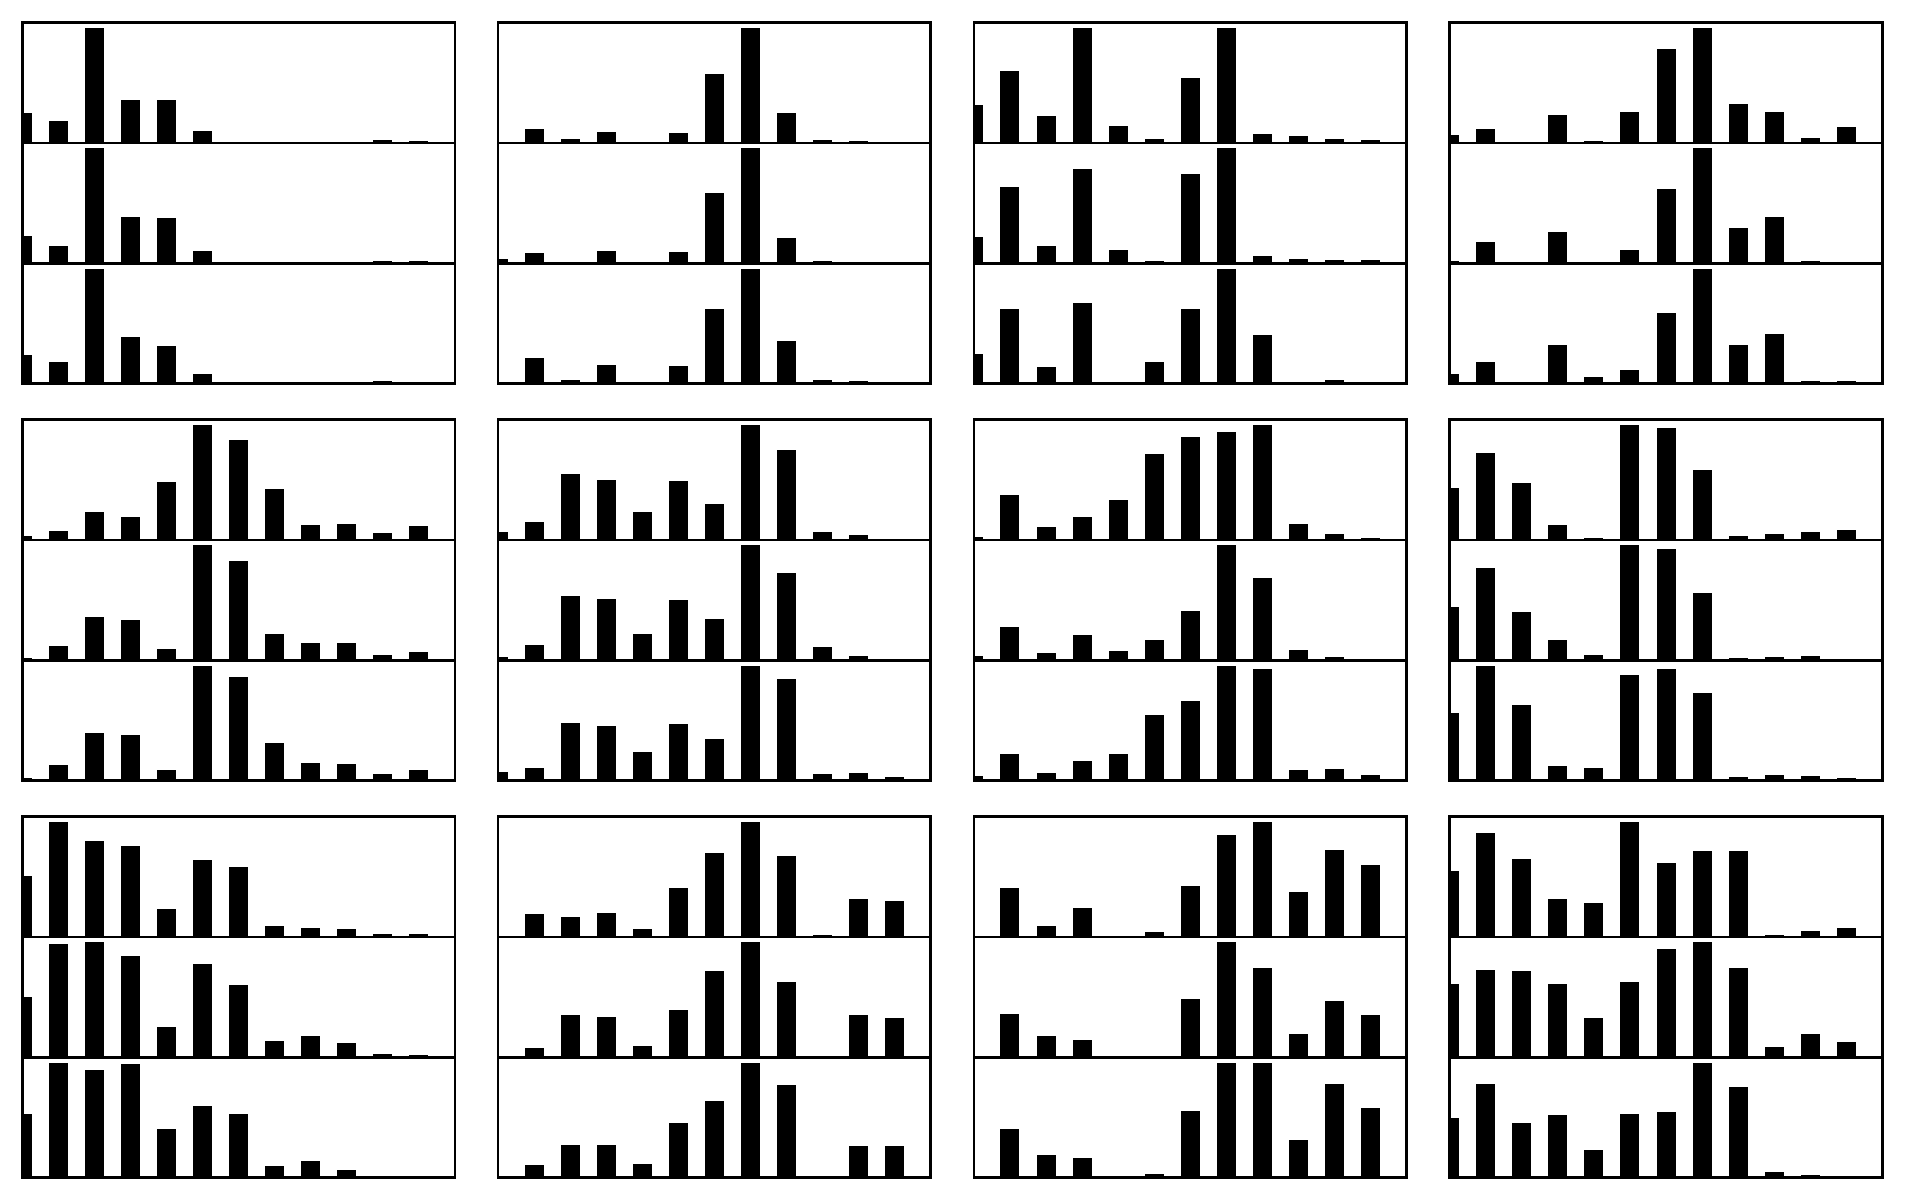
\includegraphics[height=8cm]{ms_cnn_features}
  \caption{基于CNN的多尺度故障诊断方法提取的特征向量}
  \label{fig:ms_cnn_features}
\end{figure}

可以看出,与图~\ref{fig:cnn_features}中使用单一尺度网络结构的故障诊断模型提取的特征向
量相比,使用本章中基于多尺度网络的故障诊断模型提取的特征在类别之间具有更好的区分性,
而同一类样本之间的相似程度也更高。

可以看出,与图~\ref{fig:average_pooling_features}中显示的使用单层平均值下采样提取的
特征向量相比,使用本章中的特征提取方法获得的结果的类内相似性和类间区分性更高。

表~\ref{tab:chap4:ref_comparison}给出了近些年发表的文献中使用多尺度故障诊断方法的诊断
效果。虽然前两种多尺度故障诊断方法都能达到100\%的预测精度,但是其考虑的故障类别相对较
小,而且测试集的样本数量也很少,代表性不足。与在其他几种多尺度故障诊断方法相比,本章中
提出的基于CNN的多尺度故障诊断方法测试的样本数更多,考虑的故障类型更全面,达到的预测精
度也更高。
\begin{table}[htb]
  \centering
  \begin{minipage}[t]{0.9\linewidth}
  \caption{不同多尺度方法诊断效果比较}
  \label{tab:chap4:ref_comparison}
    \begin{tabularx}{\linewidth}{lXXX}
      \toprule[1.5pt]
        方法描述 & 测试样本数 & 故障类别数 & 测试准确率 \\
      \midrule[1pt]
        MSE + SVM~\cite{zhengjinde2012mse}     & 45    & 3  & 1.0000 \\
        MFE + SVM~\cite{zhengjinde2014mfe}     & 40    & 4  & 1.0000 \\
        CMFE + SVM~\cite{zhengjinde2016cmfe}   & 42    & 6  & 0.9760 \\
        MPE + HMM~\cite{zhao2015rolling}       & 120   & 4  & 0.9420 \\
        LMD + MSE + PNN~\cite{mengzong2016lmd} & 300   & 10 & 0.9870 \\
        MS-CNN                                 & 10119 & 12 & 0.9985 \\
      \bottomrule[1.5pt]
    \end{tabularx}
    \footnotesize
    MPE:多尺度置换熵,HMM:隐马尔可夫模型,LMD:局部平均分解,PNN:概率神经网络
  \end{minipage}
\end{table}

\section{小结}

本章首先对上采样做了简单的介绍,然后在第~\ref{cha:chapter3}章基于CNN的网络结构的基础上,
引入了上采样层,并通过上采样操作,使得经过下采样的整体特征和下采样前的局部特征能够进行
融合。此外,本章通过一种递归的过程,构建了一个能够融合多种尺度下特征的网络模块,并基于
该网络模块设计了一个故障模式分类模型,实现了对信号片段的特征提取和分类。本章提出的基于CNN
的多尺度故障诊断方法在CWRU滚动轴承数据的测试集上能够达到99.85\%的预测精度,与其他一些
常见的多尺度故障诊断方法相比,在诊断精度上有非常明显的优势。
